\documentclass[a4paper]{article}
\usepackage[warn]{mathtext}
\usepackage[utf8]{inputenc}
\usepackage[T2A]{fontenc}
\usepackage[english,russian]{babel}
\usepackage{booktabs}
\usepackage{multicol}
\usepackage{fancyhdr}
\usepackage{graphicx}
\usepackage{microtype}
\usepackage{wrapfig}
\usepackage{amsmath}
\usepackage{floatflt}
\usepackage{geometry} \geometry{verbose,a4paper,tmargin=2cm,bmargin=2cm,lmargin=1.5cm,rmargin=1.5cm}
\usepackage{float}
\usepackage{amssymb}
\usepackage{caption}
\usepackage{epsfig}
\usepackage{newunicodechar}

\begin{document}

\graphicspath{ {pictures/} }
\begin{center}
    {\scshape\Large Лабораторная работа по твердотельной электронике} \par

    \

    {\huge\bfseries № 10: Горячие электроны в полупроводниках} \par 

    \

    {\large Яромир Водзяновский Б04-852}
\end{center}

\

\
\textbf{Цель работы:} Изучить влияние сильного электрического поля на элктропроводность полупроводников и эффекты, связанные с возникновением отрицательной дифференциальной провдимости при 
разогреве электронов. Определить частоту СВЧ-волны, генерируемой диодом Ганна. 


\section{Экспериментальаня установка}

\begin{figure}[H]
    \begin{center}
        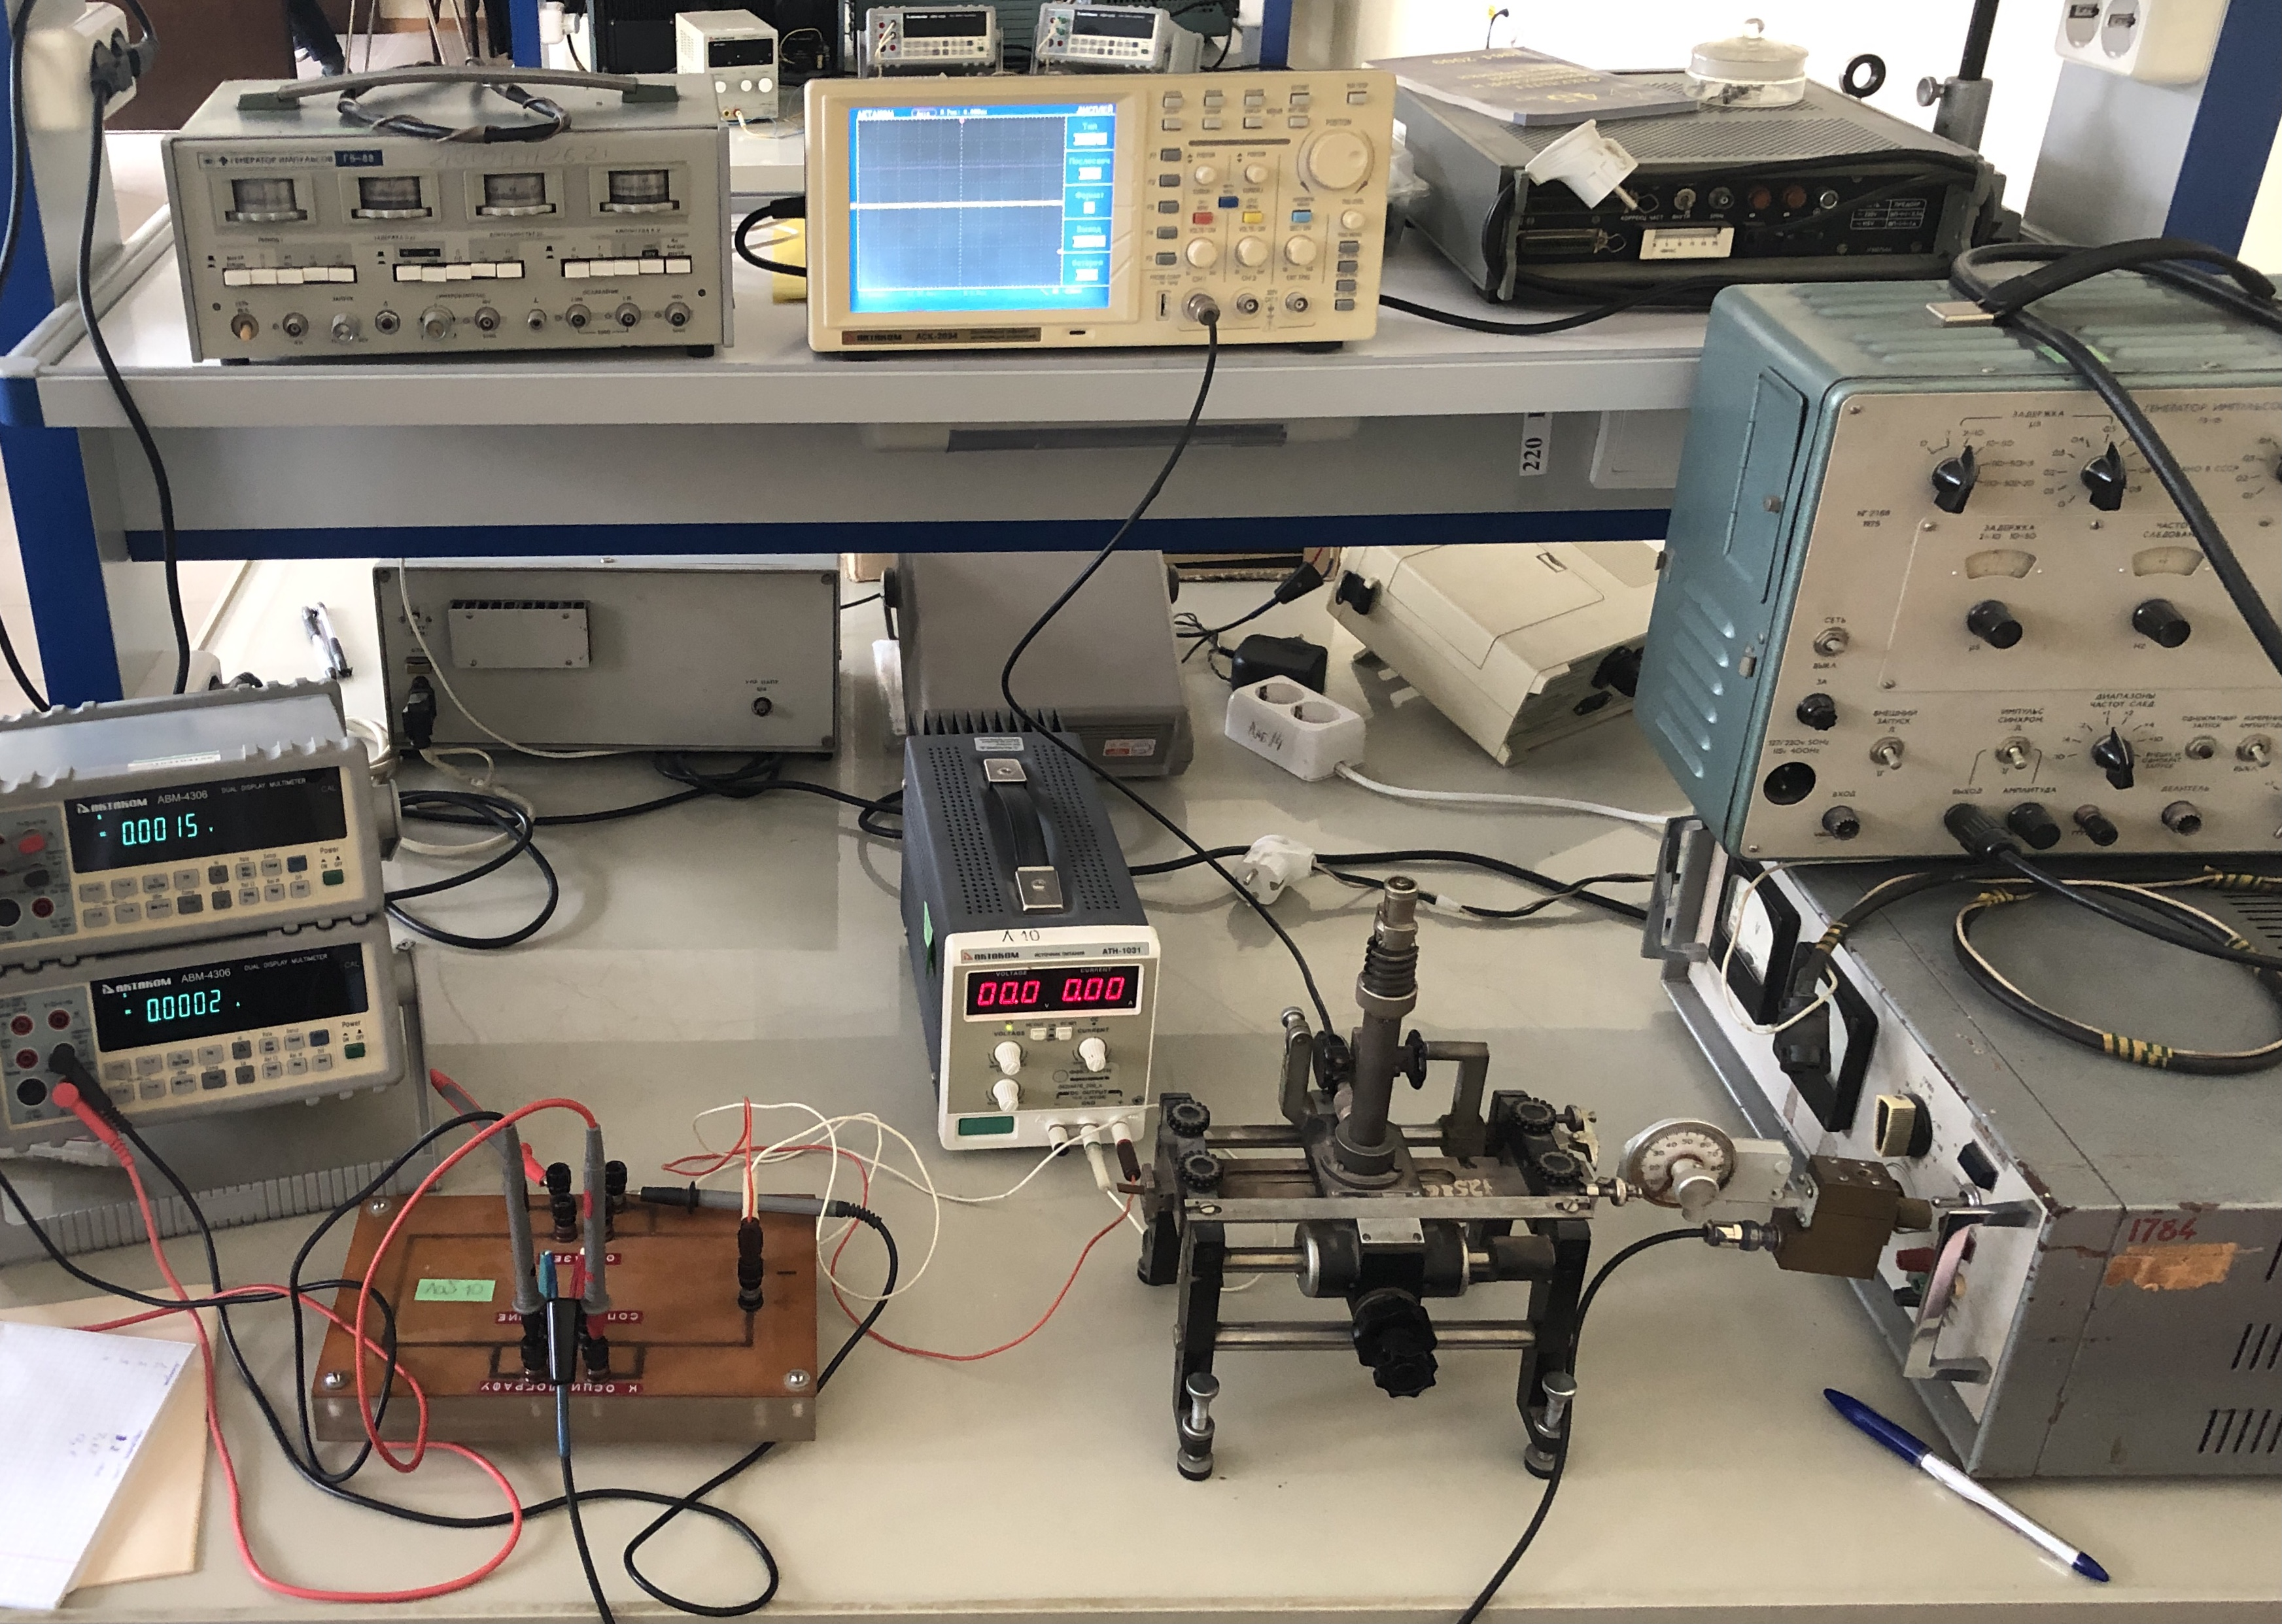
\includegraphics[scale = 0.1]{setup.jpg}
        \caption{Изображение установки}
        \label{setup}
    \end{center}
\end{figure}

На рис.\ref{setup} изображена установка, диод Ганна питается от источника постоянного напряжения, к которому подключены 
амепрметр и вольтметр. Диод подключен к волноводу, по которому бежит СВЧ-волна.

\section{Выполнение работы}

\begin{enumerate}
   
\item Вращая миллиметровую ручку будет менять положение детектора в волноводе, будем <<ловить>> пучности и записывать значение координаты 
и номер пучности в таблицу \ref{t1}. 

\begin{table}[H]
    \begin{center}
        \begin{tabular}{|c|c|c|c|c|c|c|c|}
            \hline
            № пучности & 1& 2 & 3& 4&5&6&7 \\ \hline
            Координата, мм & 3.20&7.65&12.10&16.55&21.00&25.15&30.00 \\ \hline
        \end{tabular}
        \caption{}
        \label{t1}
    \end{center}
\end{table}

\item Сделаем линейную аппроксимацию рис. \ref{p1}, коэффициенты занесем в таблицу \ref{coeffs_table}

\begin{table}[H]
\centering
\caption{Коэффициенты аппроксимации}
\label{coeffs_table}
\begin{tabular}{lrrr}
\toprule
coeffs &  coeffs\_values &  standard error &  relative se, \% \\
\midrule
   a\_0 &      4.461E+00 &       3.571E-02 &       8.006E-01 \\
   a\_1 &     -1.279E+00 &       7.143E-01 &       5.587E+01 \\
\bottomrule
\end{tabular}
\end{table}


\begin{figure}[H]
    \begin{center}
        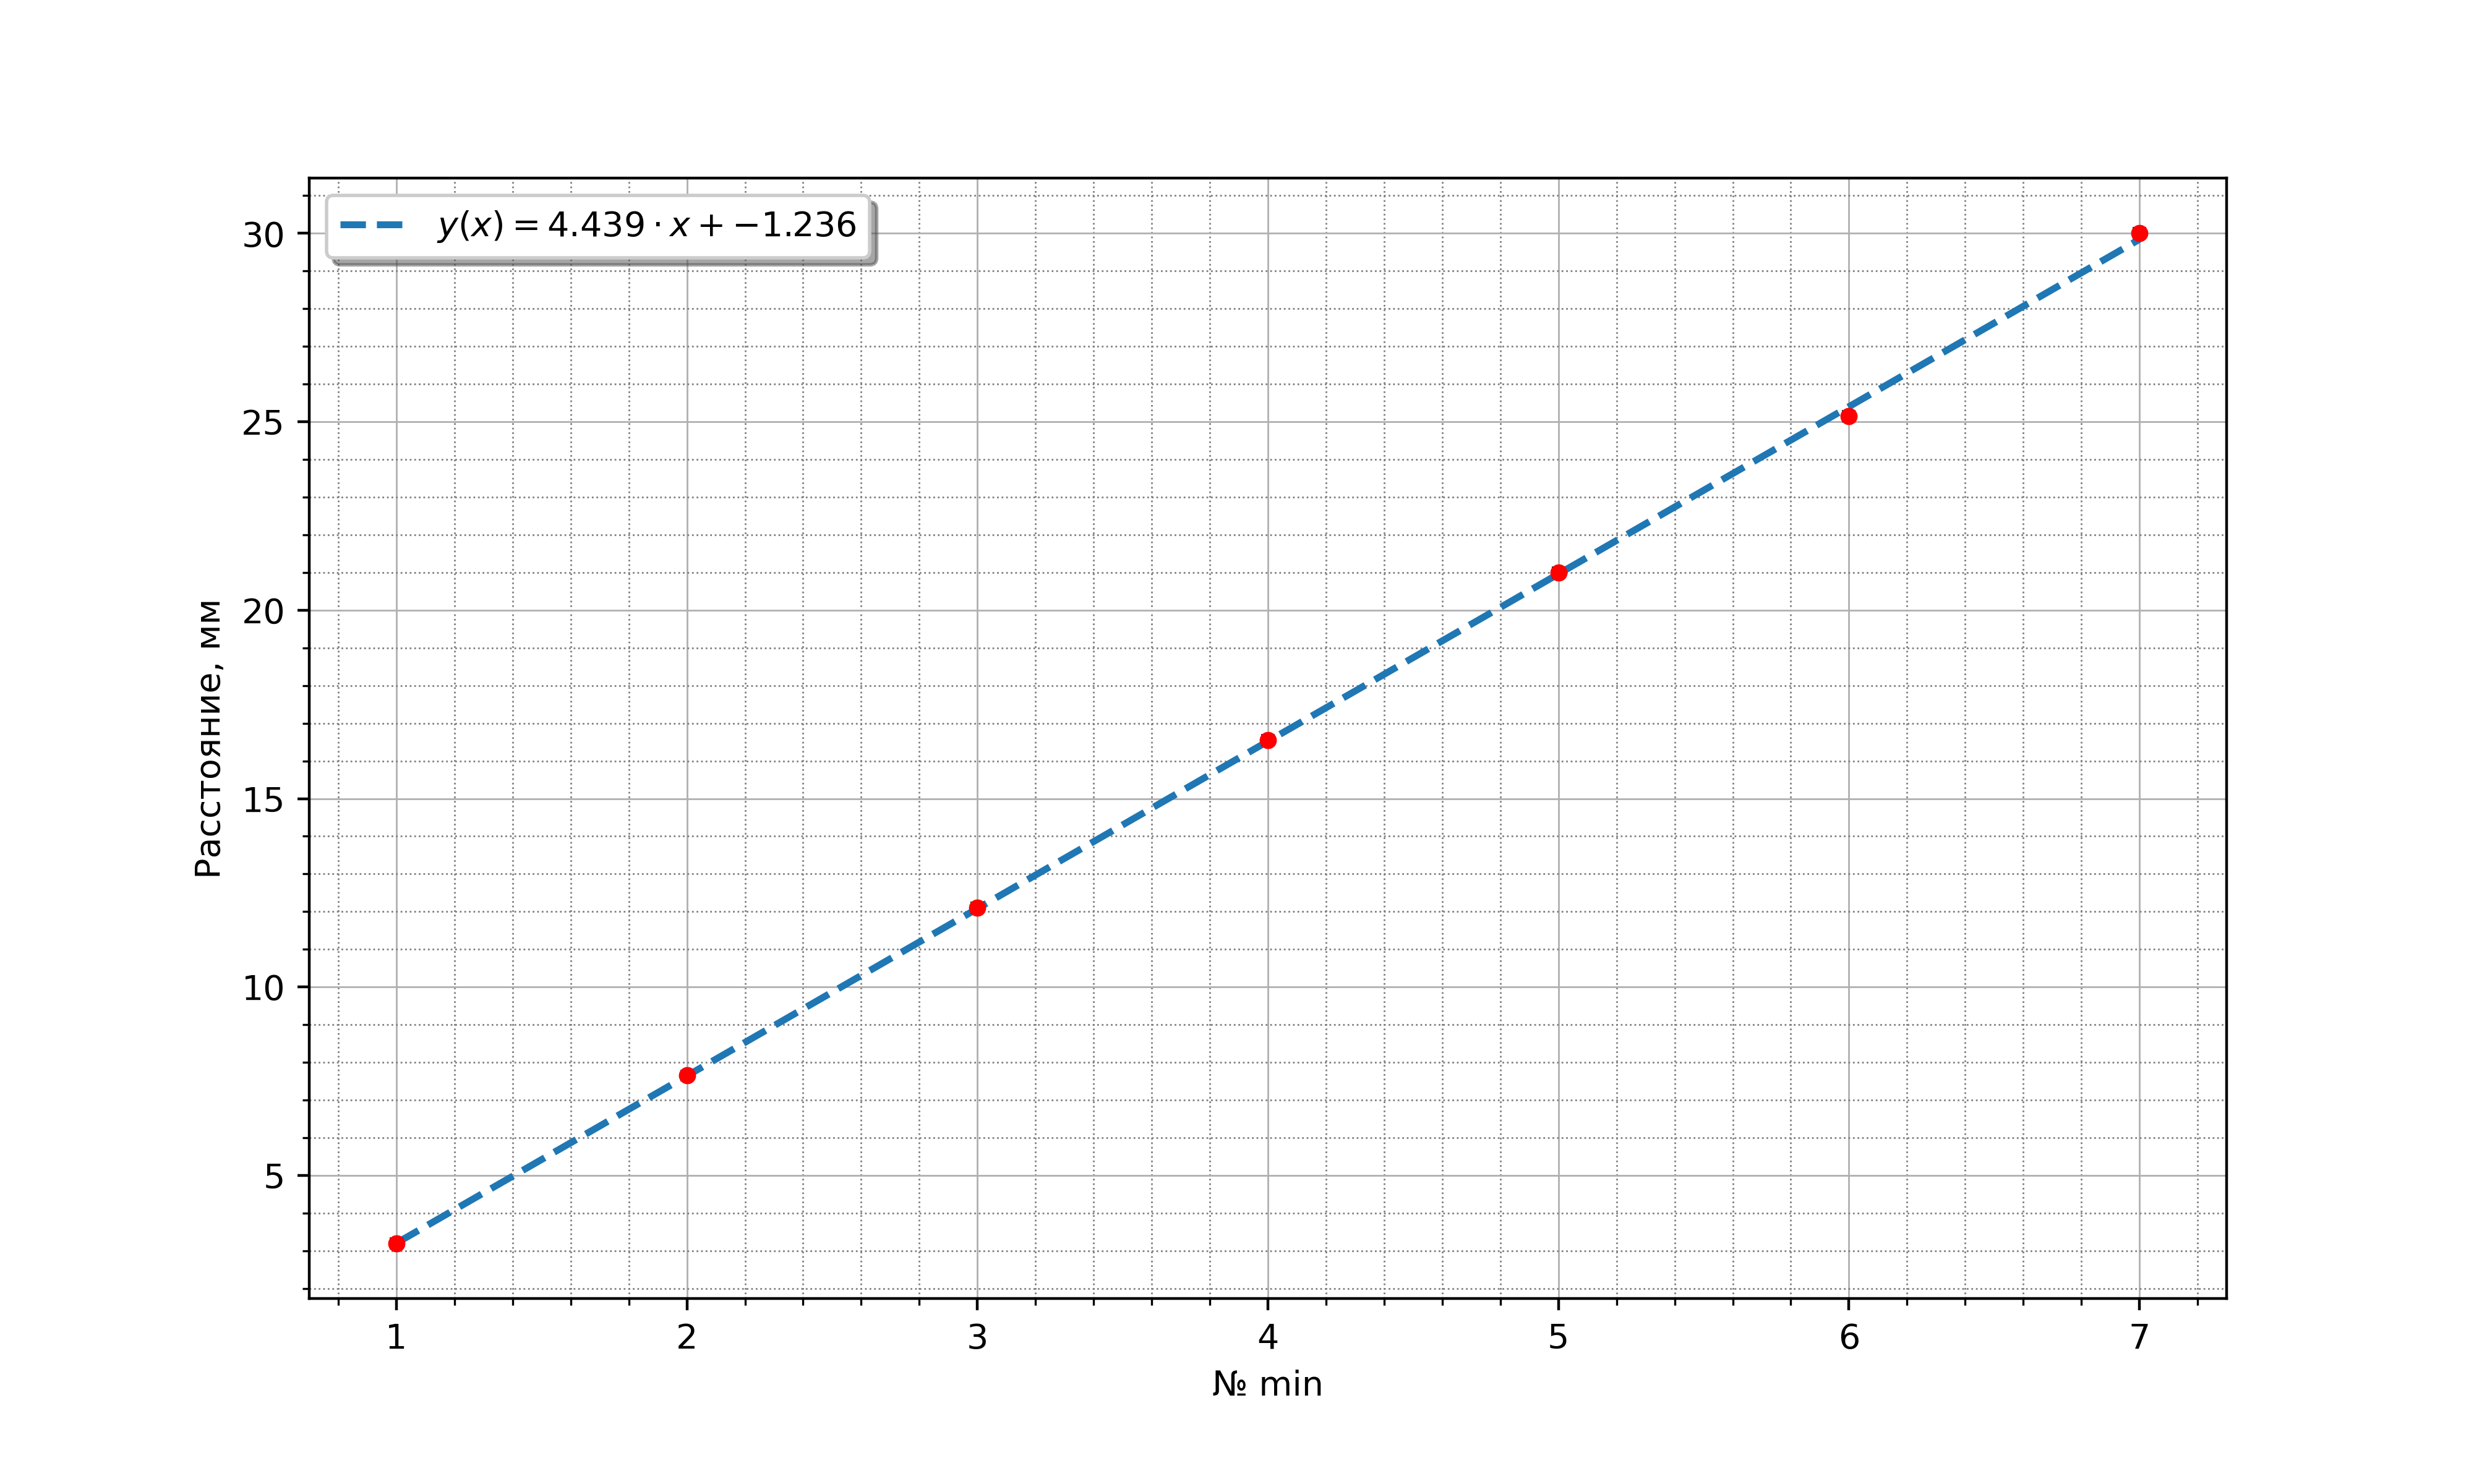
\includegraphics[scale = 0.7]{gr1.png}
        \caption{Зависимость координаты от номера пучности}
        \label{p1}
    \end{center}
\end{figure}

\item Посчитаем дллину волны и частоту. 

\begin{center}
    \fbox{$\lambda = 2\cdot a_0 = 8.92 \pm 0.07 (мм)$}
\end{center}

\begin{center}
    \fbox{$\nu = \frac{c}{\lambda} = 33.63 \pm 0.27 (ГГц)$}
\end{center}

\end{enumerate}


\textbf{Вывод:} В ходе работы определили, что диод Ганна генерирует СВЧ излучение с частотой 33.63 ГГц.


\end{document}